\section{Introduction}

How biology produces robust patterns in space and time is still largely an open question~\parencite{scholes2017three}.
In 1952, Alan Turing proposed a mechanism referred to as Turing patterns or diffusion-driven instabilities, which explains how a homogeneous tissue results in self-organized spatial repetitive patterns of the network’s molecules ~\parencite{Turing1952, Gierer1972}.
However, this proposed mechanism is far from real biological complexity, and suffers from fine tuning, meaning only a small subset of constrained parameters can generate these spatial patterns.
Additionally, the diffusion-driven instability is based on linear stability analysis theory meaning natural relevant phenomena such as multistability, growth, exotic boundary conditions and non-linearities are often not addressed.
A way forward to understanding the relationship between theoretical Turing patterns and real biological patterns is to engineer these reaction-diffusion networks in biofilms using synthetic biology ~\parencite{Sekine2018, Karig2018}.
This would allow us to better understand the role of Turing patterns in biological pattern formation, as well as to engineer synthetic patterns for industrial applications~\parencite{cao2017programmable, tan2018polyamide,din2020interfacing}.
This approach was recently extended and implemented in~\cite{Oliver2023} where a Turing gene circuit was introduced in growing \textit{E.coli} colonies producing fluorescent periodic spatial patterns. Fig.~\ref{fig1}A,B shows a final snapshot of a bacterial colony with periodic patterns in the GFP channel and the mean fluorescence in a cross section of the colony.
Understanding how patterns arise in this realistic biological system is crucial for engineering synthetic patterning and to further understand the mechanisms of pattern formation in biology.

A realistic mathematical description of such a biological system has non-linearities, multistability, growth and boundary conditions which are not easily captured with linear stability analysis. The latter technique only describes the onset of pattern formation, not the final pattern.
Several studies have explored how these phenomena affect Turing pattern formation including non-linearities~\parencite{ermentrout1991stripes}, multistability~\parencite{Krause2023}, boundaries~\parencite{Arcuri1986,Maini1993, Maini1997,Krause2020, Krause2021, Woolley2022} and growth~\parencite{gaffney2010, Klika2017, Krause2019}.
However, these studies are often based on idealised domains, certain types of popular or convenient boundary conditions, and artificial growth assumptions.
Additionally, often they do not provide statistics of how Turing patterns become more or less robust to the fine-tuning problem when introducing these phenomena by conducting high-throughput parameter scans.
Therefore, a high-throughout numerical study is needed to understand how all these natural phenomena affect Turing pattern formation, in particular in a synthetic system such as the one in~\cite{Oliver2023}.

In this paper, we combine linear stability analysis and numerics, to study a simple Turing reaction-diffusion network with non-linearities which leads to multistability.
Our analysis goes beyond classical Turing patterns as we also consider other types of instabilities such as Hopf and Turing-Hopf and how these can generate periodic stationary or non-stationary patterns.
We find that switching of steady states in multistable system can generate unexpected outcomes not predicted by linear stability analysis.
Additionally, growth and realistic boundary conditions are added to understand how patterning occurs in microbial colonies with synthetic Turing gene circuits (see Fig.~\ref{fig1}B-C).
We find that different boundaries and growth regimes can break or form patterns, therefore adding or removing robustness to pattern formation.
Studying how all these biological phenomena affect patterning is extremely important not only in the context of engineering patterns in synthetic biology, but also to understand how robust patterns occur in developmental biology where large gene-regulatory networks commonly exhibit non-linearities and multistability and where tissues are growing while in contact with an external environments.


% Place figure captions after the first paragraph in which they are cited.
\begin{figure}[H]
    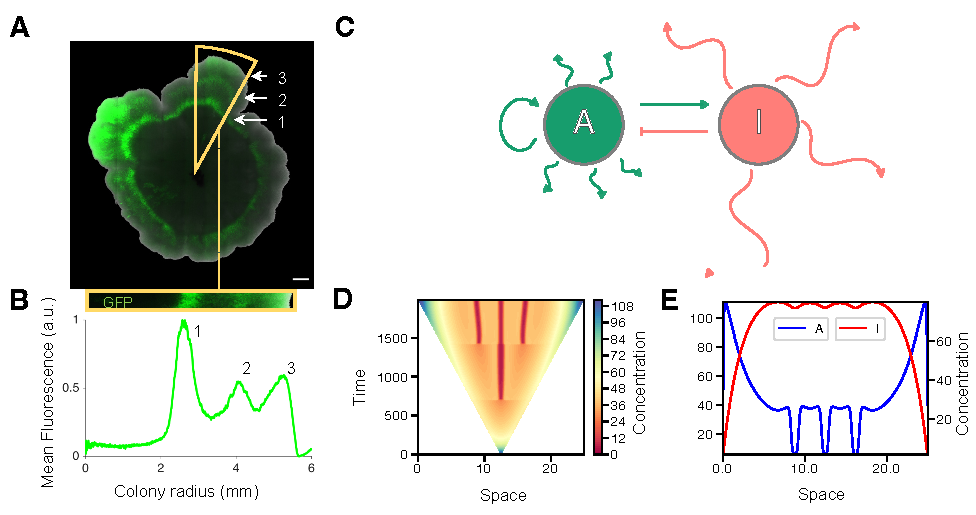
\includegraphics[width=1\textwidth]{figures/biological_example}

    \caption{{\bf Synthetic Turing patterns from experiments and theory.}
        \textbf{(A)} Last frame of a time lapse a bacterial colony grown a with synthetic 6-node Turing gene circuit producing periodic spatial patterns in two-dimensions (Scale bar: 1mm). Only GFP channel shown (\cite{Oliver2023}). \textbf{(B)} Mean fluorescence radial profile of the colony along the highlighted wedge (yellow triangle). \textbf{(C)} Two-node network based on Turing’s original paper. Slow diffusing activator in green and fast diffusor inhibitor in pink. \textbf{(D)} Kymograph of a numerical solution in 1D of the Turing circuit shown in C. Domain is growing with absorbing boundaries at the edges. Plotted as a timeseries of molecule $U$. The $Y$ axis is time (h), $X$ axis is space (mm) and concentration is shown by color with blue being high concentration and red being low concentration. A periodic pattern appears as the tissue grows. \textbf{(E)} Final snapshot of solution in D shows periodic pattern. The $Y$ axis is concentration (nM) of $U$ (left, blue) and $V$ (right, red) while the $X$ axis is space (mm). }
    %TODO figure caption
    \label{fig1}
\end{figure}
